\section{Transliteration with WFST}

\subsection*{Goal}

Transliteration is to ``spelling out'' a word in another alphabet, i.e., replace the characters with phonetic approximations, by mapping strings in one set to another set.

Weighted finite-state transducers is a probabilistic model that map strings from input vocabulary to output vocabulary. The number of states of our modeled language is finite, and the transition is weighted. Each transition is labeled by an input character, an output character and a weight. If the transition does not include the output character, then it is a weighted finite-state acceptor.

\subsection*{The probabilistic model for transition sequences}
Let $\pi$ be a path that generates the input sequence $X$ and output sequence $Y$. By definition, $\score(\pi)=\sum_i \score(\pi_i)$. Therefore, $p(y\mid x)=\frac{1}{Z} \sum_\pi \exp(\sum_i \score(\pi_i))$, where $Z$ is a sum over the whole output space which is infinite.

\subsection*{Floyd-Warshall Algorithm to compute the shortest path for all pairs in the graph without negative cycles}

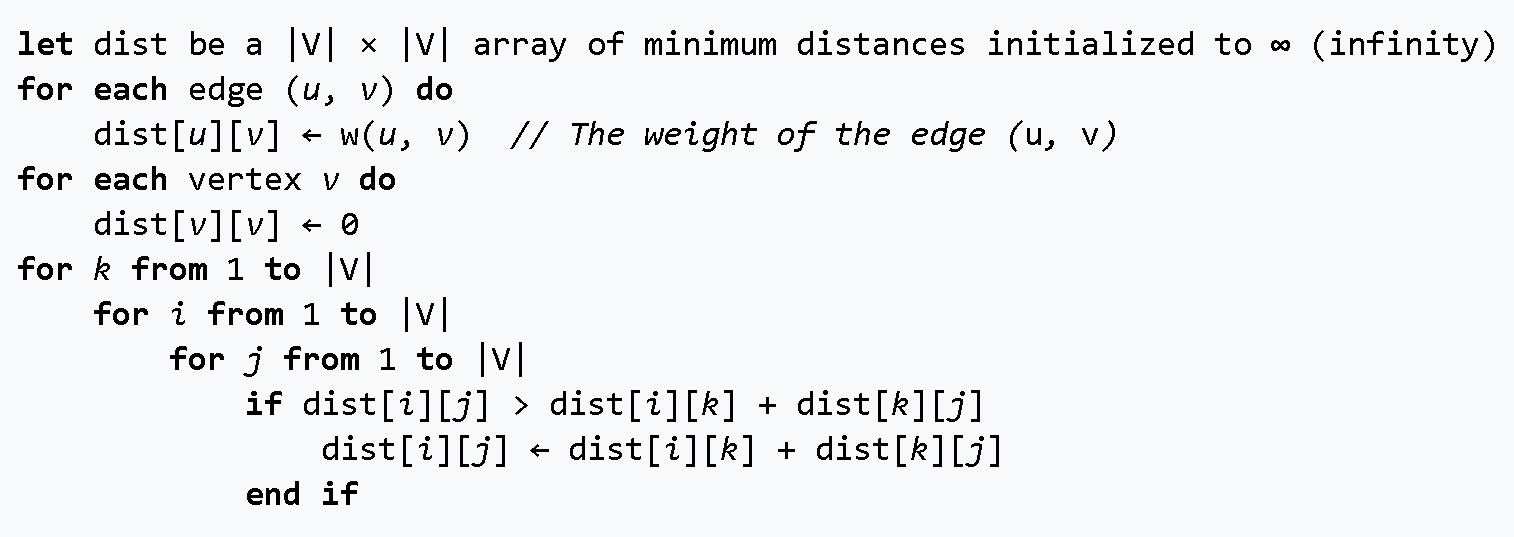
\includegraphics[width=\columnwidth]{img/Floyd_Warshall.png}

$dist^k$ naturally encodes the shortest path between two nodes of maximum length $k$.

\subsection*{Normalizer computation}

Let $\mathbb{\alpha}$ be the vector of weights of starting in the states and $\mathbb{\beta}$ be the vector of weights of ending in the states. Let $W^{\omega}$ be a matrix s.t. $W_{nm}^{\omega}$ is the weight from $n$ to $m$ with arc labeled by $\omega$, $\omega$ is an element of output space. Then $Z=\alpha^T (\sum_{\omega\in \Omega\cup \{\epsilon\}} W^{\omega})^* \beta$, where the $*$ (Kleene closure) is computed by Floyd-Warshall using semiring $(R^+\cup\{+\infty\}, \min, +, +\infty, 0)$.